\documentclass[a4paper, 12pt]{article}
\usepackage{comment} % enables the use of multi-line comments (\ifx \fi) 
\usepackage{lipsum} %This package just generates Lorem Ipsum filler text. 
\usepackage{fullpage} % changes the margin
\usepackage[utf8]{inputenc}
\usepackage[]{algorithm2e}
\usepackage{graphicx}

\begin{document}
%Header-Make sure you update this information!!!!
\noindent
\large\textbf{Documentação TP0} \hfill \textbf{Ícaro Harry} \\
\normalsize AEDS3 \hfill  Matrícula: 2014033050\\


\section{Introdução}
\paragraph{}
O problema proposto pelo TP0 foi a implementação de um Treap, que é uma estrutura de dados composta pela mistura de outras duas estruturas de dados: \textit{heap} e \textit{binary search tree} (árvore binária de pesquisa). O Treap possui tanto as propriedades de uma árvore binária de pesquisa quanto as de um heap, ou seja, um nó possui um ponteiro para o nó a sua esqueda, que deve possuir um valor \textbf{menor} do que ele e um ponteiro para o nó a sua direita que deve possuir um valor \textbf{maior} do que ele. 
Além disso, cada nó possui uma prioridade, que, para respeitar a propriedade de um \textit{heap}, deve ser menor nos filhos. Em outras palavras, os nós para quais um pai aponta, devem possuir uma prioridade maior do que a dele.
\paragraph{}
O desafio da implementação consistia em realizar as operações padrões de estruturas de dados de \textit{inserção} e \textit{remoção}, por meio de outras duas operações: o \textit{corte} e a \textit{fusão}.

\section{Modelagem do Problema}
\paragraph{}
Para a implementação de um treap da maneira como foi proposta, as principais operações a serem feitas são o \textit{corte} e a \textit{fusão}.

\subsection{Corte}
\paragraph{}
A operação de corte consiste em receber um valor e um treap e parti-lo em dois. O primeiro contendo apenas nós com valores menores ou iguais ao valor dado e o segundo contendo apenas nós com valores maiores ao valor dado. Para essa operação, não é necessário considerar a prioridade, pela definição dada, precisamos considerar apenas o valor de cada nó.
\paragraph{}
Pela definição de uma árvore binária de pesquisa, é comum realizar operações recursivas nessa estrutura de dado, por serem de mais fácil implementação. Por esse motivo, optei em buscar uma solução recursiva para o problema.
\paragraph{}
Para chegar a solução, analisei a formação de diferentes treaps. Dessa maneira, percebi que deveria fazer diferentes operações, caso fosse para a esquerda ou para a direita da árvore. A solução encontrada, por essa análise foi próxima a uma busca em uma árvore binária de pesquisa, com a diferença que, quando o valor do nó for menor do que o "buscado", liga-se o nó na árvore de elementos menores ou iguais ao valor "buscado". E, quando for maior, liga-se o nó na árvore de elementos maiores.


\subsection{Fusão}
\paragraph{}
A operação de fusão consiste no inverso do corte. Ao receber dois treaps, um contendo nós com valores menores ou iguais à um dado valor, e outro contendo nós com valores maiores do que o valor dado, deve-se retornar a união entre ambos os treaps.
\paragraph{}
Pelo mesmo motivo citado na subseção anterior, optei por buscar uma solução recursiva para o problema.
\paragraph{}
Encontrei a solução, dessa vez, pensando na prioridade de cada nó. Considerando que a árvore a esquerda possui somente elementos menores do que a árvore a direita, pode-se concluir que qualquer nó da árvore maior sempre entrará o mais a direita da árvore menor. E, da mesma forma, qualquer elemento da árvore menor entrará o mais a esquerda da árvore maior. Dessa forma, caminha-se pela árvore da direita, só para os nós a sua esquerda, e na árvore da esquerda só para os nós a sua direita. Sendo assim, começando pelas raízes, caminha-se na árvore da esquerda procurando um elemento que possua prioridade maior do que o nó da árvore a direita. Quando encontrar esse elemento, liga-se a árvore da direita ao nó que apontava para ele e insere, recursivamente, esse elemento na árvore da direita, repetindo a operação. Quando chegar à folha, conclui-se que todos os elementos estão em suas devidas posições.
\paragraph{}
Em minha implementação, encontrei alguns problemas de performance, que fizeram a fusão ter um pior desempenho que o corte, pois sempre verifico se o treap está no caminho certo, através de uma variável auxiliar que guarda a direção. Além disso, utilizo uma função auxiliar para trocar os valores dos nós, no momento em que encontra o nó de prioridade maior.


\subsection{Inserção}
\paragraph{}
É possível realizar a inserção de um nó com valor x e prioridade y facilmente utilizando as operações de corte e fusão. Basta cortar o treap em duas árvores, uma com nós menores do que x e outra com nós maiores. Após isso realiza-se uma fusão de x com a primeira árvore e uma fusão da árvore resultada da operação anterior e a árvore de elementos maiores do que x.




\subsection{Remoção}
\paragraph{}
Também é possível realizar a remoção de um nó com valor x, utilizando corte e fusão. Para isso, corta-se o treap em 3: um com elementos menores do que x, outro contendo apenas x e o terceiro contendo elementos maiores do que x. Após isso, basta unir o primeiro ao terceiro.

\section{Análise Teórica do Custo Assintótico de Tempo}
\paragraph{}
O custo assintótico de tempo pode ser analizado considerando-se as propriedades de uma árvore binária de pesquisa. Onde, no caso médio, quando ela está balanceada, ela possui altura log(n). Dessa maneira, para acessar qualquer elemento, deve-se percorrer log(n) elementos. Caso a árvore esteja desbalanceada, pode chegar no pior caso a altura n.
\subsubsection{Corte}
\paragraph{}
Sendo assim, a operação de corte, deve percorrer todos os elementos até a folha, e para cada elemento determinar e ele é menor ou igual ou maior do que o valor dado. Por isso, se a árvore estiver balanceada, temos um custo assintótico O(log n). Por outro lado, se a árvore estiver desbalanceada, pode atingir altura n, comportando-se de forma parecida a uma simples lista encadeada. Nesse caso, a operação de corte terá complexidade de O(log n).
\subsubsection{Fusão}
\paragraph{}
A operação de fusão, assim como o corte, também depende da altura da árvore. Já que ela caminha sempre nos elementos das extremidades internas do treap, ela irá depender da altura desses galhos. Em uma árvore balanceada, com altura log(n), a complexidade da fusão também será O(log n), pelo mesmo motivo do corte. No caso de uma árvore desbalanceada, ela pode também, chegar ao máximo de O(n).


\section{Análise Prática (Experimentos)}
\paragraph{}
Pela análise experimental, pude confirmar o comportamento logaritmico das funções. Executei os testes em um computador com processador Intel i5 e 4gb de memória RAM. Em meus testes, a remoção foi executada de maneira consideravelmente mais rápida do que a inserção. Isso ocorreu devido a utilização do sistema operacional no momento do teste. Entretanto, percebe-se o comportamento logarítmico em ambos os casos.
\begin{figure}
\caption{Inserção}
 \centering % para centralizarmos a figura
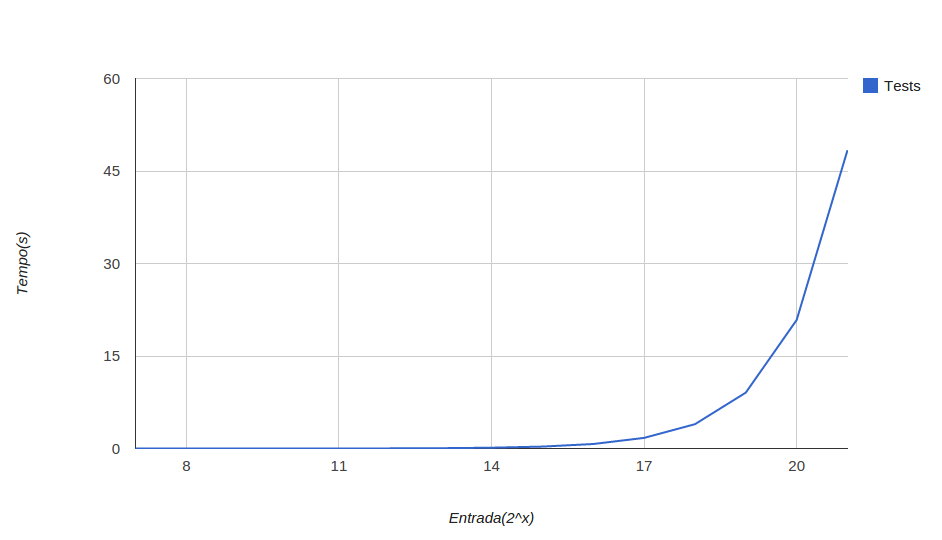
\includegraphics[width=15cm]{char_insert.png} % leia abaixo
\label{figura:ins}
\end{figure}
\begin{figure}
\caption{Remoção}
 \centering % para centralizarmos a figura
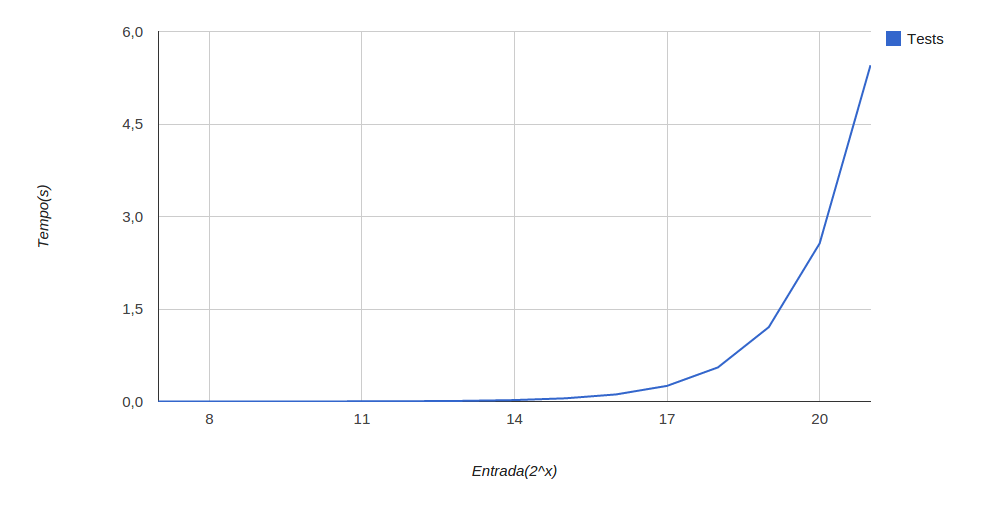
\includegraphics[width=15cm]{char_remv.png} % leia abaixo
\label{figura:rem}
\end{figure}
\begin{figure}
\caption{Corte}
 \centering % para centralizarmos a figura
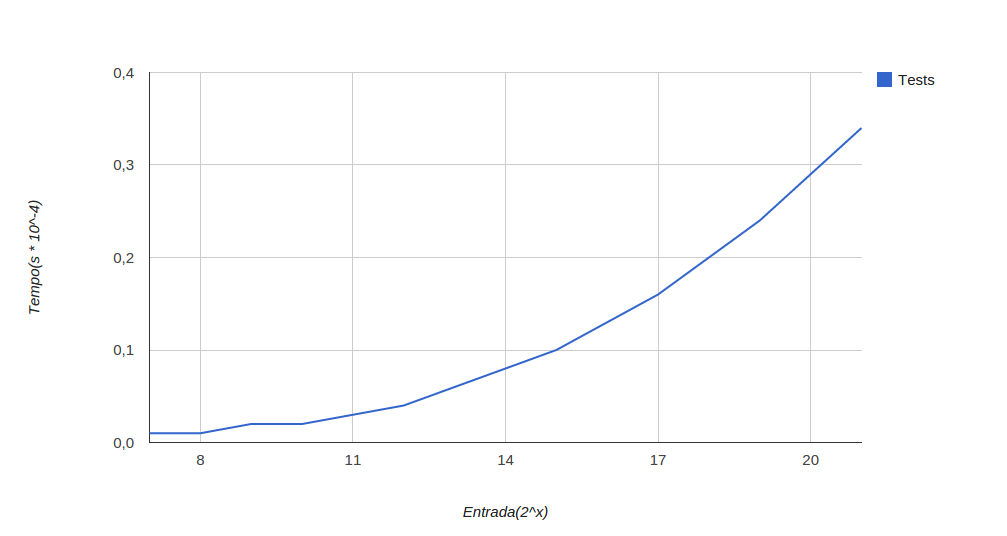
\includegraphics[width=15cm]{char_split.png} % leia abaixo
\label{figura:rem}
\end{figure}
\begin{figure}
\caption{Fusão}
 \centering % para centralizarmos a figura
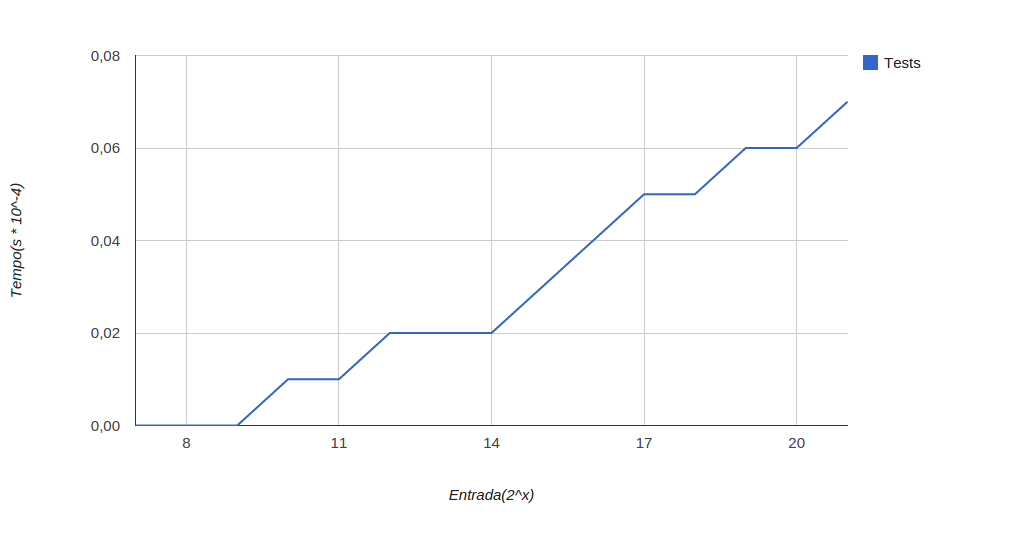
\includegraphics[width=15cm]{char_merge.png} % leia abaixo
\label{figura:rem}
\end{figure}

\section{Conclusão}
\paragraph{}
Por meio da implementação desse Trabalho Prático, conclui-se que o treap é uma estrutura de dados que pode possuir aplicações práticas interessantes. Por ter propriedades tanto de uma árvore binária de pesquisa, quanto de um heap, ele se encontra, na maior parte dos casos, balanceado, o que gera um ganho de performance e evita operações de balanceamento da árvore, que podem ser muito custosas.
\paragraph{}
A implementação das operações de inserção e remoção utilizando corte e fusão, geraram uma maior facilidade de implementação, pois, dessa maneira, utilizando-se das propriedades conhecidades das árvores binárias de pesquisa, pôde-se chegar em simples soluções recursivas.

\end{document}
